\documentclass[10pt]{article}
\usepackage{hyperref}
\usepackage[T1]{fontenc}
\usepackage[latin1]{inputenc}
%\usepackage{beton}
%\usepackage{ccfonts}
%\usepackage{concrete}
\usepackage{concmath}
\usepackage{eulervm}
\usepackage{amsmath,amsthm,amssymb}
\usepackage{mathtools}
\usepackage{multicol}
\usepackage{marginnote}
\usepackage{pgfplots}
\usepackage{float}
\usepackage{hyperref}
\pgfplotsset{compat=1.5}
\usepackage{graphicx}
\graphicspath{ {./images/} }
\usepackage{listings}
\usepackage{xcolor}
\definecolor{codegreen}{rgb}{0,0.6,0}
\definecolor{codegray}{rgb}{0.5,0.5,0.5}
\definecolor{codepurple}{rgb}{0.58,0,0.82}
\definecolor{backcolour}{rgb}{0.95,0.95,0.92}
\lstdefinestyle{mystyle}{
    backgroundcolor=\color{backcolour},   
    commentstyle=\color{codegreen},
    keywordstyle=\color{magenta},
    numberstyle=\tiny\color{codegray},
    stringstyle=\color{codepurple},
    basicstyle=\ttfamily\footnotesize,
    breakatwhitespace=false,         
    breaklines=true,                 
    captionpos=b,                    
    keepspaces=true,                 
    numbers=left,                    
    numbersep=5pt,                  
    showspaces=false,                
    showstringspaces=false,
    showtabs=false,                  
    tabsize=2
}

\lstset{style=mystyle}

\usepackage{mathtools}

\usepackage{wasysym}
\usepackage[margin=1.5in]{geometry} 
\usepackage{enumerate}
\index{\usepackage}\usepackage{multicol}

\newcommand{\N}{\mathbf{N}}
\newcommand{\Z}{\mathbb{Z}}

\newcommand{\R}{\mathbf{R}}
\newcommand{\C}{\mathbf{C}}
\newcommand{\Pbb}{\mathbb{P}}
\newcommand{\Fcal}{\mathcal{F}}
\newcommand{\Acal}{\mathcal{A}}
\newcommand{\Ecal}{\mathcal{E}}
\newcommand{\Ebb}{\mathbb{E}}
\newcommand{\Qbb}{\mathbb{Q}}

\newenvironment{theorem}[2][Theorem]{\begin{trivlist}
  \item[\hskip \labelsep {\bfseries #1}\hskip \labelsep {\bfseries #2.}]}{\end{trivlist}}
\newenvironment{lemma}[2][Lemma]{\begin{trivlist}
  \item[\hskip \labelsep {\bfseries #1}\hskip \labelsep {\bfseries #2.}]}{\end{trivlist}}
\newenvironment{exercise}[2][Exercise]{\begin{trivlist}
  \item[\hskip \labelsep {\bfseries #1}\hskip \labelsep {\bfseries #2.}]}{\end{trivlist}}
\newenvironment{reflection}[2][Reflection]{\begin{trivlist}
  \item[\hskip \labelsep {\bfseries #1}\hskip \labelsep {\bfseries #2.}]}{\end{trivlist}}
\newenvironment{proposition}[2][Proposition]{\begin{trivlist}
  \item[\hskip \labelsep {\bfseries #1}\hskip \labelsep {\bfseries #2.}]}{\end{trivlist}}
\newenvironment{corollary}[2][Corollary]{\begin{trivlist}
  \item[\hskip \labelsep {\bfseries #1}\hskip \labelsep {\bfseries #2.}]}{\end{trivlist}}

\newenvironment{definition}[2][Definition]{\begin{trivlist}
  \item[\hskip \labelsep {\bfseries #1}\hskip \labelsep {\bfseries #2.}]}{\end{trivlist}}

\begin{document}
	
  \renewcommand{\qedsymbol}{\smiley}
	\title{Optimal Decision Making \\ Report}
	\author{Aurelien Debbas, Marijn van der Meer, Hugo Bassas}
	
	\maketitle

\section{Mean Absolute Error Penalised Regression}

\begin{figure}[!ht]
  \centering
  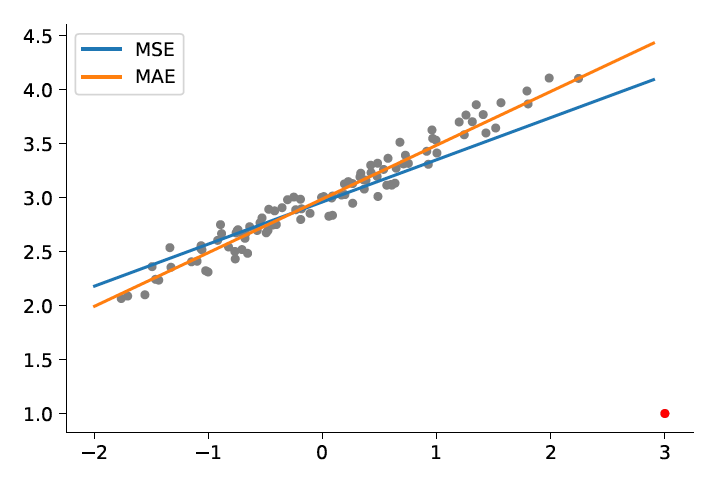
\includegraphics[width=0.5\textwidth]{doc/images/im1_.png}
  \caption{Figure 1: MSE vs. MAE estimators for a dataset with 1 outlier (red dot). }
  \vspace{-3mm}
  \label{fig:mae-mse}
\end{figure}

  \begin{exercise}{1} 
  (5 points).
  Figure~\ref{fig:mae-mse} visualizes the outputs predicted by the MSE
and MAE estimators on a dataset with 1 outlier. Explain the difference between the two estimators intuitively. Hint: Compare how Eq.~\ref{eq:mse} and Eq.~\ref{eq:mae} penalise errors. 

\begin{equation}\label{eq:mse}
    \hat\theta_{MSE} = arg min_\theta \frac{1}{N} \sum_{i=1}^N(y^{(i)}-\theta^Tx^{(i)})^2
\end{equation}

\begin{equation}\label{eq:mae}
    \hat\theta_{MAE} = arg min_\theta  \frac{1}{N} \sum_{i=1}^N|y^{(i)}-\theta^Tx^{(i)}|
\end{equation}


\textit{Answer.} The MSE estimator is computed from the sum of squared distances between our target variables $y^{(i)}$ and predicted values $\hat y^{(i)} = \theta^Tx^{(i)}$ while MAE uses the sum of absolute differences i.e., the average magnitudes of errors. MSE is more easy to use in optimisation problems because it is convex while MAE is not and has the same gradient everywhere. But MAE is more robust to outliers as can be seen in Fig.~\ref{fig:mae-mse}. This is due to the fact that MSE squares errors, and thus for an outlier we have that $e^2 >> |e|$. When searching for optimal weights $\hat\theta$, MSE will have a tendency to try to adjust in a way of minimising big errors such as the one outlier in our case. In our case, this explains why the model predicted using MSE (in blue) is closer to the outlier than the one from MAE (in red). 
  \end{exercise}

\begin{exercise}{2}
In case of high-dimensional inputs (d > N), it makes sense to seek a sparse
parameter vector $\theta$. This means that many components of $\theta$ should be zero. The non-zero components of $\theta$ then correspond to the key features or key inputs that have a significant impact on the outputs. Sparsity can be induced by adding an L1-penalty to the objective function of Eq.~\ref{eq:mse} or Eq.~\ref{eq:mae}, which yields the least absolute
shrinkage and selection operator (LASSO) method of regression analysis. In case of the MAE objective, the resulting LASSO estimator satisfies:
\begin{equation}\label{eq:lasso}
    \hat\theta_{lasso} = arg min_\theta  \frac{1}{N} \sum_{i=1}^N|y^{(i)}-\theta^Tx^{(i)}| + \lambda ||\theta||_1 
\end{equation}
In practice, $\lambda$ is a hyperparameter typically chosen by cross validation. That is, we randomly partition D into a training dataset $D_{train}$
and a validation dataset $D_{val}$. We then solve Eq.~\ref{eq:lasso} using only $D_{train}$ for different
values of $\lambda$ and select the estimator that has minimal MAE on $D_{val}$. Rewrite Eq.~\ref{eq:lasso} as a linear program (not necessarily in standard form).

\textit{Answer.} 
We write $\Lambda = [\lambda_1, ... , \lambda_k]$ the set of all values we choose for the hyperparameter $\lambda$. We also note $x_i\in \mathbb{R}^d \; \forall i=1 ,\dots, N$. Then for $\lambda\geq 0$, LASSO regression finds $\theta \in \mathbb{R}^d$ such that   

\begin{equation}
\begin{array}{ll@{}lll}
\text{min} &\displaystyle\sum\limits_{i=1}^{N} & |y_i-\theta^Tx_i| + &\lambda\displaystyle\sum\limits_{i=1}^{d}|\theta_i|
\end{array}
\end{equation}

With the addition of auxiliary variables $z_i$ and $\delta_i$, we use the fact that $|y_i - \theta^T x_i| < z_i$ is equivalent to $-z_i < y_i - \theta^T x_i  < z_i$. Now minimising the sum of $z_i$ is equal to minimising the sum of $ |y_i-\theta^Tx_i|$ because $\sum\limits_{i=1}^{N}  |y_i-\theta^Tx_i| < \sum\limits_{i=1}^{N} z_i$. The same applies to $|\theta_i|$. So we can write the following linear program:
\begin{equation*}
\begin{array}{lll@{}lll}
&\text{min}  &\displaystyle\sum\limits_{i=1}^{N}z_i +  \lambda\sum\limits_{i=1}^{d}\delta_i &\\
\text{subject to} 
&& y_i-\theta^Tx_i &\leq z_i && i=1 ,\dots, N \\
&& -y_i+\theta^Tx_i &\leq z_i && i=1 ,\dots, N \\
                 && \theta_i &\leq \delta_i &&  i=1 ,\dots, d \\
                && -\theta_i &\leq \delta_i &&  i=1 ,\dots, d 
\end{array}
\end{equation*}
To rewrite this in standard form we introduce slack variables $s,t,u,v$: 
\begin{equation*}
\begin{array}{lll@{}lll}
&\text{min}  &\displaystyle\sum\limits_{i=1}^{N}z_i +  \lambda\sum\limits_{i=1}^{d}\delta_i &\\
\text{subject to} 
&& -\theta^Tx_i - z_i + s &= y_i && i=1 ,\dots, N \\
&& +\theta^Tx_i -z_i + t &= y_i && i=1 ,\dots, N \\
                 && \theta_i - \delta_i + u&= 0  &&  i=1 ,\dots, d \\
                && -\theta_i - \delta_i + v &= 0  &&  i=1 ,\dots, d 
                \\
                && s,t,u,v &\geq 0  && 
\end{array}
\end{equation*}



\end{exercise}
  

  \section*{Appendix}
\newpage  
 \begin{thebibliography}{9}

\end{thebibliography}
 
\end{document}

